\chapter{Materiais e Métodos}

\section{Construção da Ferramenta}


Dois equipamentos comerciais foram utilizados para construção da ferramenta de coleta sincronizada: Mindwave Mobile II e o
GP3; para a coleta de EEG e ET, respectivamente. O código de coleta que gera o dataset
multimodal foi construído em MATLAB, e o pré-processamento dos dados antes de serem \textit{inputs} no treinamento
de algoritmos no software Orange foi construído em Python. O presente capítulo irá apresentar os equipamentos de coleta
e o método adotado para construção da ferramenta. 

\subsection{Mindwave Mobile II}
O equipamento possui um eletrodo de coleta e um eletrodo de referência que ficam posicionados 
acima da sobrancelha esquerda e na orelha esquerda do participante, respectivamente. 
A posição do eletrodo de coleta em relação ao sistema de referência de posição de eletrodos (10-20), é o FP1, 
correspondendo a região Frontopolar 1. A coleta de dados do aparelho se dá por conexão via \textit{bluetooth} e 
funciona em computadores Mac, Windows ou celulares Androids ou iOS, disponíveis em um raio de 10 metros (informações do fabricante). 
Ele coleta ondas cerebrais variando entre 3 e 100Hz, com uma frequência de 512Hz (NeuroSky Inc., 2015). 

O aparelho automaticamente distingue os dados coletados em ondas alfa, beta, gama, teta e delta; 
além de coletar informações subjetivas no formato de medidas de atenção e meditação, 
por meio de um algoritmo de reforço de aprendizado não disponibilizado ao publico. 
Também mede a ativação muscular próxima ao eletrodo para estimar a qualidade do sinal. 
O MindWave Mobile filtra interferência elétrica e converte o sinal detectado pelo eletrodo em sinal digital. 
O chip que faz o filtro e conversão se chama ThinkGear, e permite a filtragem de ruído para interferência ativação muscular (EMG) e 50/60Hz de corrente alternada. 

\subsection{Gazepoint GP3}

O GP3 é um equipamento comercial de coleta do movimento dos olhos, 
fabricado pela Gazepoint. Possui software próprio para análise dos dados, 
além de ser possível realizar coleta de dados com linguagens de programação open-source. O GP3 funciona emitindo uma luz infravermelha (IR) 
diretamente nos olhos do participante e captando a reflexão da luz para localizar o ponto focal ao longo do tempo. 
Permite coletar a direção do olhar, número de fixações, tempo até a primeira fixação, taxa de piscadas,
 duração de piscadas, diâmetro da pupila, tempo de duração do olhar em um determinado ponto focal, 
 objetos observados em uma imagem, entre outros (informações do fabricante).

O Gazepoint GP3 estabelece sua conexão com o computador através de dois cabos USB - um cabo de energia e outro para dados.
Seu posicionamento ideal é logo abaixo do monitorde estímulo. Para um melhor posicionamento, o fabricante 
sugere uma distância ideal de 65 cm dos olhos do participante até o equipamento. O GP3 possui as seguintes características, conforme
especificado pelo fabricante:

\begin{itemize}
    \item Acurácia de 0.5-1 grau de ângulo visual
    \item 60 Hz de frequencia de atualização
    \item calibração de 5 e 9 pontos
    \item API
    \item Captura movimento de 25cm horizontais e 11cm verticais
    \item 15 cm de limite de profundidade de movimento
\end{itemize}

Para poder realizar a coleta dos dados, é necessário manter o Gazepoint Control (API do desenvolvedor) ligado. 

\subsubsection{Calibração GP3}
Uma calibração é realizada pela própria API do equipamento, afim de estabelecer qual o apontamento ocular do participante. 
A calibração pode ser feita em 5 pontos ou 9 pontos no monitor de exibição de estímulo. Os pontos na tela são apresentados
em sequencia e o participante deve acompanha-los com o olhar até a finalização da calibração. Após a calibração ser concluída, a API calcula o erro do sistema em relação ao olhar para o olho esquerdo (em verde) 
e direito (vermelho). 

\subsubsection{Dados Capturados pelo GP3}

\textbf{Fixação:} É um agrupamento de pontos focais do olhar que duram entre 20-300 ms (Brand, 2020). \textbf{Gaze Point:} Gaze point é o ponto focal do usuário em um dado momento. No equipamento GP3 é gravado um ponto focal a cada aproximadamente 17 milisegundos.
O ponto de gaze é gravado em relação as coordenadas x e y, que servem para identificar a posição do olhar na tela de experimento. 
\textbf{Sacada:} Compreende a um movimento rápido dos olhos após a fixação, e pode ser medida através de pixels por segundo.
O valor limite entre sacada e fixação é a velocidade de 1.8 pixels por segundo (George e Routray, 2016), onde acima
é uma sacada e abaixo, uma fixação.
%Anjith George and Aurobinda Routray, “A score level fusion method for eye movement biometrics,” Pattern Recognition Letters, vol. 82, pp. 207–215, 2016





\section{Coleta}
Para a coleta simultânea, duas linguagens de programação foram utilizadas: MATLAB e Python. 
A montagem do \textit{setup} foi feita com base nas coletas realizadas para a construção dos datasets EEGEyeNet e 
 ZuCO. Inicialmente, o software Gazepoint Control foi ligado para rodar em \textit{background} no computador. 
Em seguida, o MindWave mobile II foi ligado e teve sua conexão \textit{bluetooth} estabelecida e verificada.
A porta de conexão (porta COM) PC-Mindwave pode mudar, então foi verificado em qual porta foi estabelecida a conexão 
em todo início de nova coleta. Após a verificação da porta, foi observado se houve necessidade ou não de alterar
este valor na variável do código. O Gazepoint
  ficou distante do participante até o software próprio acusar distância ideal
   (sinalizado por um sinal verde no topo do software de regulação do equipamento). 
   Para teste de coleta foram utilizados dois monitores: um para calibração e apresentação de imagens, 
   e outro para o desenvolvimento de código e testagem (figura 6.1) 


   \begin{figure}
    \centering
    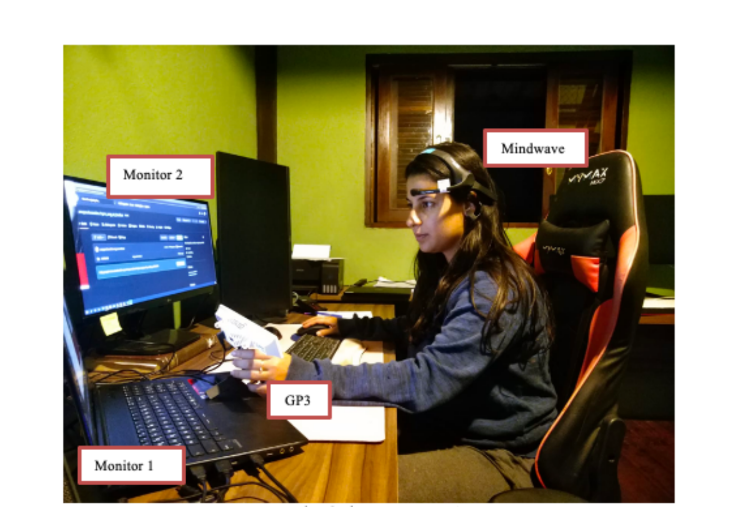
\includegraphics[width=80mm]{Screen Shot 2022-08-14 at 00.54.17.png}
    \caption{Montagem de Estudo de Caso da Ferramenta de Coleta EEG-ET.}
\end{figure}


\section{Código}

\begin{figure}
    \centering
    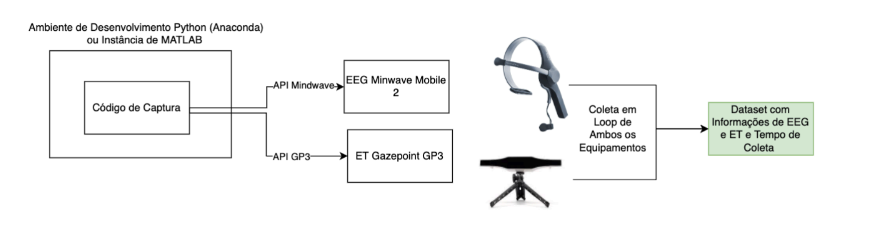
\includegraphics[width=1mm]{code_work.png}
    \caption{Montagem de Estudo de Caso da Ferramenta de Coleta EEG-ET.}
\end{figure}





%Tabela 6.1 Caracteristicas Montior utilizado na Coleta de Eye Tracking 
%Monitor	Video Interno conectado a Intel® HD Graphics 630
%Resolução da área de trabalho	1920  x 1080
%Resolução do sinal ativo	1920  x 1080
%Taxa de atualização	60 Hz
%Intensidade de bits	6 bits
%Formato de cor 	RGB
%Espaço de cores	Alcance dinâmico padrão

\section{Criação do Dataset}
O equipamento GP3 possui uma \textit{Application Programming Interface} (API) própria, 
o Open Gaze API. 
A API é uma alternativa de se controlar o equipamento sem precisar do software 
pago tambem feito pela Gazepoint. A API utiliza de um \textit{Transmission Control Protocol – Internet Protocol (TCP/IP) 
socket}, que permite a comunicação entre a aplicação e o servidor (fonte dos dados de ET). 
O IP determina o endereço para o qual os dados serão enviados, e o TCP utiliza a arquitetura de 
rede para realizar o transporte. O formato de dado utilizado para a API é o \textit{Extensible Markup Language} (XML), 
que também pode ser implementado e estabelecer conexão com Python. 
As portas utilizadas para a comunicação de forma padrão são: 
localhost (127.0.0.1) e port 4242. 

Na API do Gazepoint, o cliente tem duas tags de comunicação: GET e SET. 
Ao utilizar o SET o cliente pode alterar o valor de alguma variável. 
O comando GET não tem a possibilidade de alterção de valores. O servidor 
pode enviar dados para o cliente com diferentes tags: ACK, NACK, CAL e REC. 
As duas primeiras são geradas em resposta aos comandos de GET e SET (ACK – Sucesso e NACK –Falha). 
Os CAL são gerados com bases nas calibrações e REC serve para os dados gravados. 
Estas regras de escrita são utilizadas pelo codigo em Python para estabelecer o controle do GP3,
 permitindo que o código calibre o equipamento e estabeleça definições de variáveis.

Para o funcionamento adequado do Mindwave, é necessário instalar uma tecnologia chamada \textit{ThinkGear} (TG), 
que permite a troca de informações entre o equipamento e os softwares compativeis e processa o 
sinal detectado pelo eletrodo. O TG também é responsável pelo cálculo dos chamados \textbf{eSense Meteres}, 
correspondendo aos dados de Atenção e Meditação em uma escalda de 0 a 100 (Neurosky, 2018). 

